\section{Desarrollo/Análisis}
El diagrama de bloques generales para el funcionamiento del voltímetro es el siguiente.
\begin{figure}[H]

\centering
\tikzset{every picture/.style={line width=0.75pt}} %set default line width to 0.75pt        

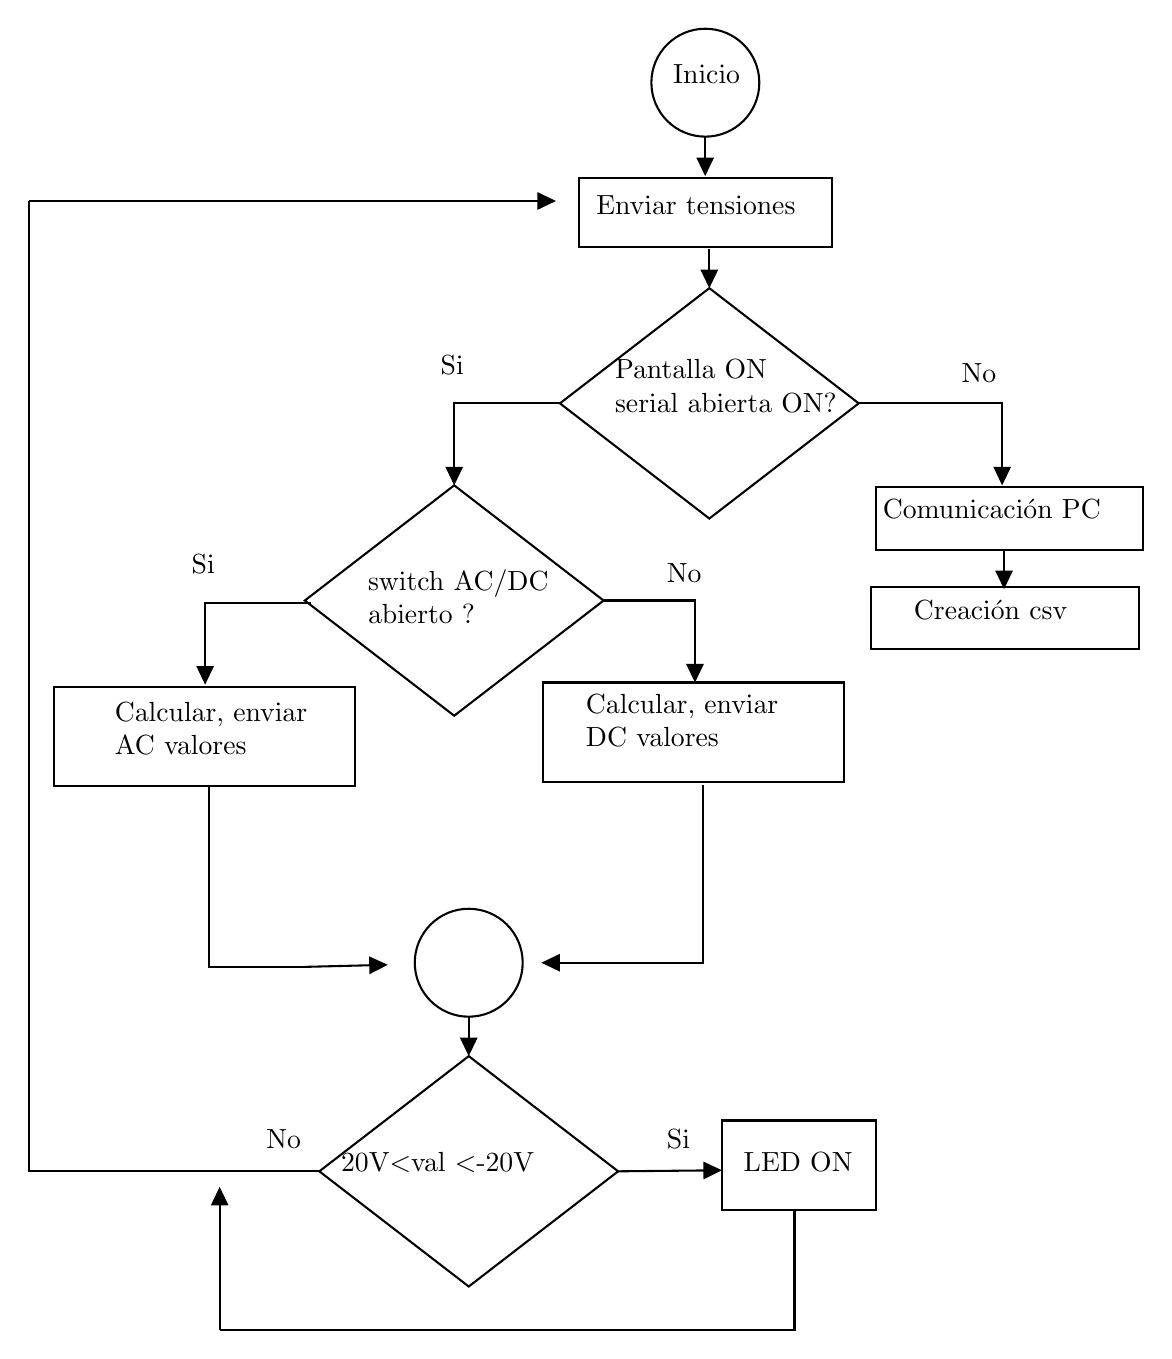
\begin{tikzpicture}[x=0.75pt,y=0.75pt,yscale=-1,xscale=1]
%uncomment if require: \path (0,736); %set diagram left start at 0, and has height of 736

%Flowchart: Connector [id:dp7813495520702245] 
\draw   (320,81) .. controls (320,66.64) and (331.64,55) .. (346,55) .. controls (360.36,55) and (372,66.64) .. (372,81) .. controls (372,95.36) and (360.36,107) .. (346,107) .. controls (331.64,107) and (320,95.36) .. (320,81) -- cycle ;
%Straight Lines [id:da8847526091998554] 
\draw    (345.92,107) -- (345.92,123) ;
\draw [shift={(345.92,126)}, rotate = 270] [fill={rgb, 255:red, 0; green, 0; blue, 0 }  ][line width=0.08]  [draw opacity=0] (8.93,-4.29) -- (0,0) -- (8.93,4.29) -- cycle    ;
%Flowchart: Process [id:dp3892985602062795] 
\draw   (285,127) -- (407,127) -- (407,160) -- (285,160) -- cycle ;
%Flowchart: Decision [id:dp21596588394867888] 
\draw   (347.92,180) -- (419.9,235.5) -- (347.92,291) -- (275.94,235.5) -- cycle ;
%Straight Lines [id:da7204417446380422] 
\draw    (347.92,161) -- (347.92,177) ;
\draw [shift={(347.92,180)}, rotate = 270] [fill={rgb, 255:red, 0; green, 0; blue, 0 }  ][line width=0.08]  [draw opacity=0] (8.93,-4.29) -- (0,0) -- (8.93,4.29) -- cycle    ;
%Straight Lines [id:da451260237829443] 
\draw    (489,256) -- (489,272) ;
\draw [shift={(489,275)}, rotate = 270] [fill={rgb, 255:red, 0; green, 0; blue, 0 }  ][line width=0.08]  [draw opacity=0] (8.93,-4.29) -- (0,0) -- (8.93,4.29) -- cycle    ;
%Straight Lines [id:da49582350632228556] 
\draw    (225,256) -- (225,272) ;
\draw [shift={(225,275)}, rotate = 270] [fill={rgb, 255:red, 0; green, 0; blue, 0 }  ][line width=0.08]  [draw opacity=0] (8.93,-4.29) -- (0,0) -- (8.93,4.29) -- cycle    ;
%Straight Lines [id:da9013438330772021] 
\draw    (153.04,507) -- (190,506.08) ;
\draw [shift={(193,506)}, rotate = 178.57] [fill={rgb, 255:red, 0; green, 0; blue, 0 }  ][line width=0.08]  [draw opacity=0] (8.93,-4.29) -- (0,0) -- (8.93,4.29) -- cycle    ;
%Straight Lines [id:da797473974800426] 
\draw    (330,505) -- (270,505) ;
\draw [shift={(267,505)}, rotate = 360] [fill={rgb, 255:red, 0; green, 0; blue, 0 }  ][line width=0.08]  [draw opacity=0] (8.93,-4.29) -- (0,0) -- (8.93,4.29) -- cycle    ;
%Straight Lines [id:da006314317293441896] 
\draw    (232,531) -- (232,547) ;
\draw [shift={(232,550)}, rotate = 270] [fill={rgb, 255:red, 0; green, 0; blue, 0 }  ][line width=0.08]  [draw opacity=0] (8.93,-4.29) -- (0,0) -- (8.93,4.29) -- cycle    ;
%Straight Lines [id:da9058055932314646] 
\draw    (303.98,605.5) -- (351,605.03) ;
\draw [shift={(354,605)}, rotate = 179.43] [fill={rgb, 255:red, 0; green, 0; blue, 0 }  ][line width=0.08]  [draw opacity=0] (8.93,-4.29) -- (0,0) -- (8.93,4.29) -- cycle    ;
%Straight Lines [id:da1932315478192832] 
\draw    (489.92,306) -- (489.92,322) ;
\draw [shift={(489.92,325)}, rotate = 270] [fill={rgb, 255:red, 0; green, 0; blue, 0 }  ][line width=0.08]  [draw opacity=0] (8.93,-4.29) -- (0,0) -- (8.93,4.29) -- cycle    ;
%Straight Lines [id:da6050013822698619] 
\draw    (20,138) -- (271,138) ;
\draw [shift={(274,138)}, rotate = 180] [fill={rgb, 255:red, 0; green, 0; blue, 0 }  ][line width=0.08]  [draw opacity=0] (8.93,-4.29) -- (0,0) -- (8.93,4.29) -- cycle    ;
%Shape: Right Angle [id:dp24954692627046726] 
\draw   (419.9,235.5) -- (489,235.5) -- (489,256) ;
%Flowchart: Process [id:dp33592140600780107] 
\draw   (428,276) -- (557,276) -- (557,306) -- (428,306) -- cycle ;
%Shape: Right Angle [id:dp2914826540765745] 
\draw   (275.94,235.5) -- (225,235.5) -- (225,256) ;
%Flowchart: Decision [id:dp9064156706798434] 
\draw   (225,275) -- (296.98,330.5) -- (225,386) -- (153.02,330.5) -- cycle ;
%Straight Lines [id:da6126735924115385] 
\draw    (341,351) -- (341,367) ;
\draw [shift={(341,370)}, rotate = 270] [fill={rgb, 255:red, 0; green, 0; blue, 0 }  ][line width=0.08]  [draw opacity=0] (8.93,-4.29) -- (0,0) -- (8.93,4.29) -- cycle    ;
%Shape: Right Angle [id:dp7943090498770735] 
\draw   (296.98,330.5) -- (341,330.5) -- (341,351) ;
%Straight Lines [id:da7128924347373624] 
\draw    (105,352) -- (105,368) ;
\draw [shift={(105,371)}, rotate = 270] [fill={rgb, 255:red, 0; green, 0; blue, 0 }  ][line width=0.08]  [draw opacity=0] (8.93,-4.29) -- (0,0) -- (8.93,4.29) -- cycle    ;
%Shape: Right Angle [id:dp8866366667209189] 
\draw   (155.94,331.5) -- (105,331.5) -- (105,352) ;
%Flowchart: Process [id:dp15212318966923655] 
\draw   (32,372) -- (177,372) -- (177,420) -- (32,420) -- cycle ;
%Flowchart: Process [id:dp5589357347254946] 
\draw   (268,370) -- (413,370) -- (413,418) -- (268,418) -- cycle ;
%Shape: Right Angle [id:dp26602461789391585] 
\draw   (153.04,507) -- (106.94,507) -- (106.94,420.5) ;
%Shape: Right Angle [id:dp9899984887472151] 
\draw   (330,505) -- (344.94,505) -- (344.94,419.5) ;
%Flowchart: Decision [id:dp9568469291538075] 
\draw   (232,550) -- (303.98,605.5) -- (232,661) -- (160.02,605.5) -- cycle ;
%Flowchart: Connector [id:dp7268194319410761] 
\draw   (206,505) .. controls (206,490.64) and (217.64,479) .. (232,479) .. controls (246.36,479) and (258,490.64) .. (258,505) .. controls (258,519.36) and (246.36,531) .. (232,531) .. controls (217.64,531) and (206,519.36) .. (206,505) -- cycle ;
%Flowchart: Process [id:dp8372151895077977] 
\draw   (354,581) -- (428,581) -- (428,624) -- (354,624) -- cycle ;
%Shape: Right Angle [id:dp04700865884221406] 
\draw   (160.02,605.5) -- (20,605.5) -- (20,138) ;
%Shape: Right Angle [id:dp6697593994914697] 
\draw   (112,682) -- (388.94,682) -- (388.94,624.5) ;
%Straight Lines [id:da9427664494344408] 
\draw    (112,682) -- (112,616) ;
\draw [shift={(112,613)}, rotate = 90] [fill={rgb, 255:red, 0; green, 0; blue, 0 }  ][line width=0.08]  [draw opacity=0] (8.93,-4.29) -- (0,0) -- (8.93,4.29) -- cycle    ;
%Flowchart: Process [id:dp6713652946060731] 
\draw   (426,324) -- (555,324) -- (555,354) -- (426,354) -- cycle ;

% Text Node
\draw (329,71) node [anchor=north west][inner sep=0.75pt]   [align=left] {Inicio};
% Text Node
\draw (292,134) node [anchor=north west][inner sep=0.75pt]   [align=left] {Enviar tensiones};
% Text Node
\draw (301,213) node [anchor=north west][inner sep=0.75pt]   [align=left] {Pantalla ON\\ serial abierta ON?};
% Text Node
\draw (430,280) node [anchor=north west][inner sep=0.75pt]   [align=left] {Comunicación PC};
% Text Node
\draw (182,314) node [anchor=north west][inner sep=0.75pt]   [align=left] {switch AC/DC\\ abierto ?};
% Text Node
\draw (287,374) node [anchor=north west][inner sep=0.75pt]   [align=left] {Calcular, enviar\\DC valores};
% Text Node
\draw (169,595) node [anchor=north west][inner sep=0.75pt]   [align=left] {20V$\displaystyle < $val $\displaystyle < $-20V};
% Text Node
\draw (363,595) node [anchor=north west][inner sep=0.75pt]   [align=left] {LED ON};
% Text Node
\draw (468,215) node [anchor=north west][inner sep=0.75pt]   [align=left] {No};
% Text Node
\draw (217,211) node [anchor=north west][inner sep=0.75pt]   [align=left] {Si};
% Text Node
\draw (326,311) node [anchor=north west][inner sep=0.75pt]   [align=left] {No};
% Text Node
\draw (97,307) node [anchor=north west][inner sep=0.75pt]   [align=left] {Si};
% Text Node
\draw (60,378) node [anchor=north west][inner sep=0.75pt]   [align=left] {Calcular, enviar\\AC valores};
% Text Node
\draw (326,584) node [anchor=north west][inner sep=0.75pt]   [align=left] {Si};
% Text Node
\draw (133,584) node [anchor=north west][inner sep=0.75pt]   [align=left] {No};
% Text Node
\draw (445,329) node [anchor=north west][inner sep=0.75pt]   [align=left] {Creación csv};


\end{tikzpicture}
\caption{Diagrama de bloques general}
\label{dia_General}
\end{figure}
Una vez que se activen alguna de las fuentes, en la pantalla PCD8544 se mostrará las magnitudes (despreciables, \SI{0.05}{\volt}) por default en cada canal, y al estar el botón de modo AC/DC en bajo por tanto, en esta pantalla se mostrarán los valores en DC, si éste se pone en alto entonces en la pantalla se mostrarán los valores rms en AC, ahora, dependiendo de las magnitudes que se ajusten en ambos modos los LEDs de alarma se encenderán o no, que al mismo tiempo se verán en la pantalla. Por último, al presionar el botón de comunicación serial, se establece la comunicación adecuada para generar el informe del archivo csv.\par
Luego, para realizar las medidas adecuadas se tuvo que realizar una función capaz de normalizar y escalar en el intervalo de rango solicitado: [-24, 24]. 
\begin{figure}[H]
\centering


\tikzset{every picture/.style={line width=0.75pt}} %set default line width to 0.75pt        

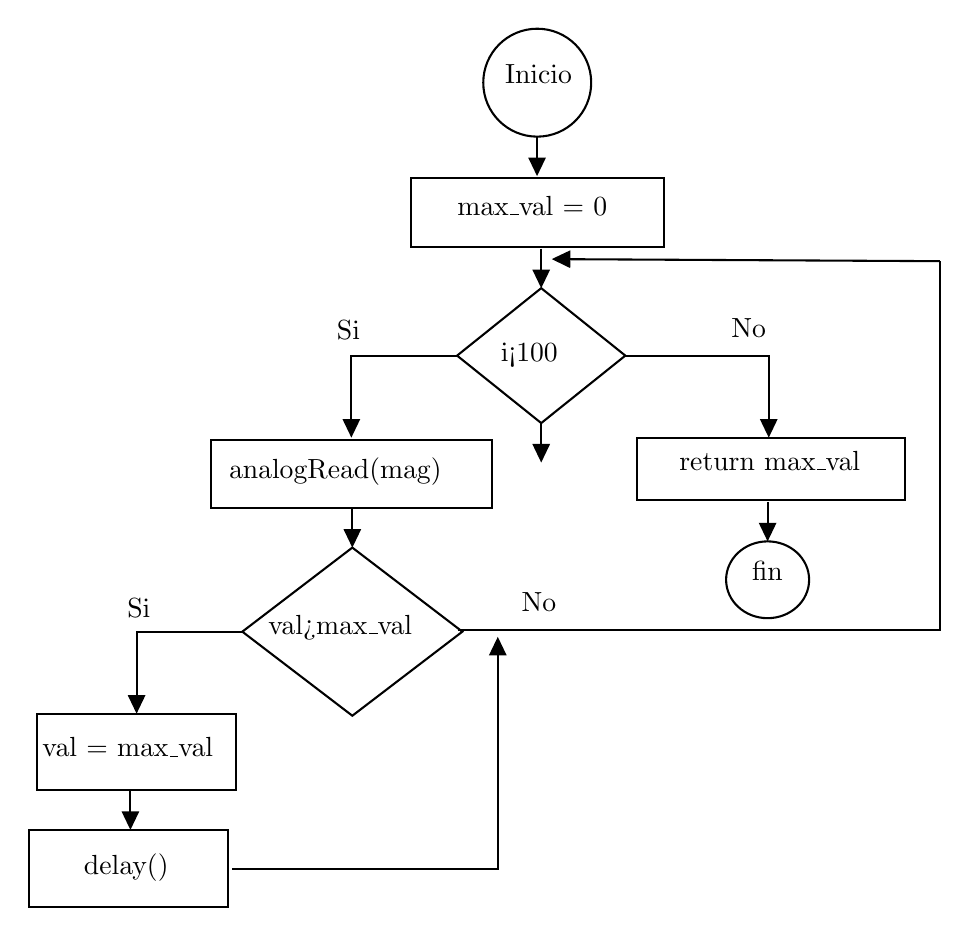
\begin{tikzpicture}[x=0.75pt,y=0.75pt,yscale=-1,xscale=1]
%uncomment if require: \path (0,491); %set diagram left start at 0, and has height of 491

%Flowchart: Connector [id:dp7813495520702245] 
\draw   (320,81) .. controls (320,66.64) and (331.64,55) .. (346,55) .. controls (360.36,55) and (372,66.64) .. (372,81) .. controls (372,95.36) and (360.36,107) .. (346,107) .. controls (331.64,107) and (320,95.36) .. (320,81) -- cycle ;
%Straight Lines [id:da8847526091998554] 
\draw    (345.92,107) -- (345.92,123) ;
\draw [shift={(345.92,126)}, rotate = 270] [fill={rgb, 255:red, 0; green, 0; blue, 0 }  ][line width=0.08]  [draw opacity=0] (8.93,-4.29) -- (0,0) -- (8.93,4.29) -- cycle    ;
%Flowchart: Process [id:dp3892985602062795] 
\draw   (285,127) -- (407,127) -- (407,160) -- (285,160) -- cycle ;
%Flowchart: Decision [id:dp21596588394867888] 
\draw   (347.92,180) -- (388.45,212.5) -- (347.92,245) -- (307.39,212.5) -- cycle ;
%Straight Lines [id:da7204417446380422] 
\draw    (347.92,161) -- (347.92,177) ;
\draw [shift={(347.92,180)}, rotate = 270] [fill={rgb, 255:red, 0; green, 0; blue, 0 }  ][line width=0.08]  [draw opacity=0] (8.93,-4.29) -- (0,0) -- (8.93,4.29) -- cycle    ;
%Straight Lines [id:da451260237829443] 
\draw    (457.55,233) -- (457.55,249) ;
\draw [shift={(457.55,252)}, rotate = 270] [fill={rgb, 255:red, 0; green, 0; blue, 0 }  ][line width=0.08]  [draw opacity=0] (8.93,-4.29) -- (0,0) -- (8.93,4.29) -- cycle    ;
%Straight Lines [id:da49582350632228556] 
\draw    (256.45,233) -- (256.45,249) ;
\draw [shift={(256.45,252)}, rotate = 270] [fill={rgb, 255:red, 0; green, 0; blue, 0 }  ][line width=0.08]  [draw opacity=0] (8.93,-4.29) -- (0,0) -- (8.93,4.29) -- cycle    ;
%Straight Lines [id:da006314317293441896] 
\draw    (327,351) -- (327,367) ;
\draw [shift={(327,348)}, rotate = 90] [fill={rgb, 255:red, 0; green, 0; blue, 0 }  ][line width=0.08]  [draw opacity=0] (8.93,-4.29) -- (0,0) -- (8.93,4.29) -- cycle    ;
%Straight Lines [id:da6050013822698619] 
\draw    (356,166.02) -- (540,167) ;
\draw [shift={(353,166)}, rotate = 0.31] [fill={rgb, 255:red, 0; green, 0; blue, 0 }  ][line width=0.08]  [draw opacity=0] (8.93,-4.29) -- (0,0) -- (8.93,4.29) -- cycle    ;
%Shape: Right Angle [id:dp24954692627046726] 
\draw   (388.45,212.5) -- (457.55,212.5) -- (457.55,233) ;
%Shape: Right Angle [id:dp2914826540765745] 
\draw   (307.39,212.5) -- (256.45,212.5) -- (256.45,233) ;
%Flowchart: Decision [id:dp9064156706798434] 
\draw   (256.92,305) -- (309.92,345.5) -- (256.92,386) -- (203.92,345.5) -- cycle ;
%Straight Lines [id:da6126735924115385] 
\draw    (457,283) -- (457,299) ;
\draw [shift={(457,302)}, rotate = 270] [fill={rgb, 255:red, 0; green, 0; blue, 0 }  ][line width=0.08]  [draw opacity=0] (8.93,-4.29) -- (0,0) -- (8.93,4.29) -- cycle    ;
%Shape: Right Angle [id:dp7943090498770735] 
\draw   (307.98,344.5) -- (540,344.5) -- (540,167) ;
%Straight Lines [id:da7128924347373624] 
\draw    (152.98,366) -- (152.98,382) ;
\draw [shift={(152.98,385)}, rotate = 270] [fill={rgb, 255:red, 0; green, 0; blue, 0 }  ][line width=0.08]  [draw opacity=0] (8.93,-4.29) -- (0,0) -- (8.93,4.29) -- cycle    ;
%Shape: Right Angle [id:dp8866366667209189] 
\draw   (203.92,345.5) -- (152.98,345.5) -- (152.98,366) ;
%Flowchart: Process [id:dp15212318966923655] 
\draw   (105,385) -- (201,385) -- (201,422) -- (105,422) -- cycle ;
%Shape: Right Angle [id:dp9899984887472151] 
\draw   (199,460) -- (327,460) -- (327,367) ;
%Flowchart: Connector [id:dp7268194319410761] 
\draw   (437,320.5) .. controls (437,310.28) and (445.95,302) .. (457,302) .. controls (468.05,302) and (477,310.28) .. (477,320.5) .. controls (477,330.72) and (468.05,339) .. (457,339) .. controls (445.95,339) and (437,330.72) .. (437,320.5) -- cycle ;
%Flowchart: Process [id:dp6713652946060731] 
\draw   (394,252) -- (523,252) -- (523,282) -- (394,282) -- cycle ;
%Straight Lines [id:da15691850789793538] 
\draw    (347.92,245) -- (347.92,261) ;
\draw [shift={(347.92,264)}, rotate = 270] [fill={rgb, 255:red, 0; green, 0; blue, 0 }  ][line width=0.08]  [draw opacity=0] (8.93,-4.29) -- (0,0) -- (8.93,4.29) -- cycle    ;
%Flowchart: Process [id:dp025828036440153967] 
\draw   (189,253) -- (324,253) -- (324,286) -- (189,286) -- cycle ;
%Straight Lines [id:da2671209465635622] 
\draw    (256.92,286) -- (256.92,302) ;
\draw [shift={(256.92,305)}, rotate = 270] [fill={rgb, 255:red, 0; green, 0; blue, 0 }  ][line width=0.08]  [draw opacity=0] (8.93,-4.29) -- (0,0) -- (8.93,4.29) -- cycle    ;
%Straight Lines [id:da2035552754915979] 
\draw    (150,422) -- (150,438) ;
\draw [shift={(150,441)}, rotate = 270] [fill={rgb, 255:red, 0; green, 0; blue, 0 }  ][line width=0.08]  [draw opacity=0] (8.93,-4.29) -- (0,0) -- (8.93,4.29) -- cycle    ;
%Flowchart: Process [id:dp8396019792624998] 
\draw   (101,441) -- (197,441) -- (197,478) -- (101,478) -- cycle ;

% Text Node
\draw (329,71) node [anchor=north west][inner sep=0.75pt]   [align=left] {Inicio};
% Text Node
\draw (306,134) node [anchor=north west][inner sep=0.75pt]   [align=left] {max\_val = 0};
% Text Node
\draw (327,205) node [anchor=north west][inner sep=0.75pt]   [align=left] {i<100};
% Text Node
\draw (215,336) node [anchor=north west][inner sep=0.75pt]   [align=left] {val>max\_val};
% Text Node
\draw (438,193) node [anchor=north west][inner sep=0.75pt]   [align=left] {No};
% Text Node
\draw (248,194) node [anchor=north west][inner sep=0.75pt]   [align=left] {Si};
% Text Node
\draw (337,325) node [anchor=north west][inner sep=0.75pt]   [align=left] {No};
% Text Node
\draw (147,328) node [anchor=north west][inner sep=0.75pt]   [align=left] {Si};
% Text Node
\draw (106.12,395) node [anchor=north west][inner sep=0.75pt]   [align=left] {val = max\_val};
% Text Node
\draw (413,257) node [anchor=north west][inner sep=0.75pt]   [align=left] {return max\_val};
% Text Node
\draw (196,260) node [anchor=north west][inner sep=0.75pt]   [align=left] {analogRead(mag)};
% Text Node
\draw (126.12,451) node [anchor=north west][inner sep=0.75pt]   [align=left] {delay()};
% Text Node
\draw (448,310) node [anchor=north west][inner sep=0.75pt]   [align=left] {fin};


\end{tikzpicture}
\caption{Diagrama de flujo función mide\_voltaje}
\label{sch3}
\end{figure}
Esta función se compone de un ciclo \texttt{for} que va iterando los valores que poseen los 4 canales y realiza una resta de 511 (la mitad de 1023) y voltaje medido, luego se hace la escala con el producto de esta substacción y la división de 48 entre 1023, todo esto para lograr manipular voltajes de \SI{0}{\volt}-\SI{5}{\volt} con el objetivo de normalizar y escalar el valor máximo medido.\par
La función para generar las alarmas tanto en DC como en AC son muy similares, por lo que el siguiente diagrama de bloques es equivalente para ambos.
\begin{figure}[H]
\centering


\tikzset{every picture/.style={line width=0.75pt}} %set default line width to 0.75pt        

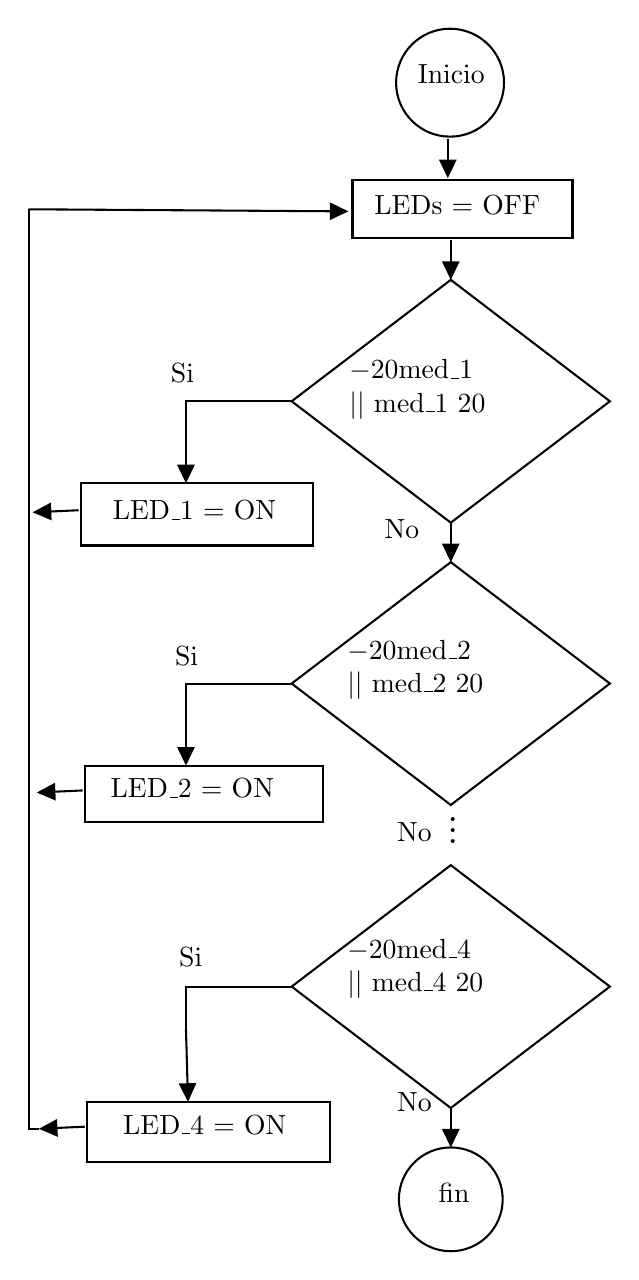
\begin{tikzpicture}[x=0.75pt,y=0.75pt,yscale=-1,xscale=1]
%uncomment if require: \path (0,689); %set diagram left start at 0, and has height of 689

%Flowchart: Connector [id:dp7813495520702245] 
\draw   (315,40) .. controls (315,25.64) and (326.64,14) .. (341,14) .. controls (355.36,14) and (367,25.64) .. (367,40) .. controls (367,54.36) and (355.36,66) .. (341,66) .. controls (326.64,66) and (315,54.36) .. (315,40) -- cycle ;
%Straight Lines [id:da8847526091998554] 
\draw    (339.92,67) -- (339.92,83) ;
\draw [shift={(339.92,86)}, rotate = 270] [fill={rgb, 255:red, 0; green, 0; blue, 0 }  ][line width=0.08]  [draw opacity=0] (8.93,-4.29) -- (0,0) -- (8.93,4.29) -- cycle    ;
%Flowchart: Decision [id:dp21596588394867888] 
\draw   (341.35,135) -- (418,193.5) -- (341.35,252) -- (264.69,193.5) -- cycle ;
%Straight Lines [id:da7204417446380422] 
\draw    (341.35,116) -- (341.35,132) ;
\draw [shift={(341.35,135)}, rotate = 270] [fill={rgb, 255:red, 0; green, 0; blue, 0 }  ][line width=0.08]  [draw opacity=0] (8.93,-4.29) -- (0,0) -- (8.93,4.29) -- cycle    ;
%Straight Lines [id:da49582350632228556] 
\draw    (213.76,214) -- (213.76,230) ;
\draw [shift={(213.76,233)}, rotate = 270] [fill={rgb, 255:red, 0; green, 0; blue, 0 }  ][line width=0.08]  [draw opacity=0] (8.93,-4.29) -- (0,0) -- (8.93,4.29) -- cycle    ;
%Straight Lines [id:da6050013822698619] 
\draw    (138,101) -- (289,101.98) ;
\draw [shift={(292,102)}, rotate = 180.37] [fill={rgb, 255:red, 0; green, 0; blue, 0 }  ][line width=0.08]  [draw opacity=0] (8.93,-4.29) -- (0,0) -- (8.93,4.29) -- cycle    ;
%Shape: Right Angle [id:dp2914826540765745] 
\draw   (264.69,193.5) -- (213.76,193.5) -- (213.76,214) ;
%Shape: Right Angle [id:dp7943090498770735] 
\draw   (142.92,544) -- (138,544) -- (138,101) ;
%Straight Lines [id:da15691850789793538] 
\draw    (162,246) -- (142.91,246.86) ;
\draw [shift={(139.92,247)}, rotate = 357.41] [fill={rgb, 255:red, 0; green, 0; blue, 0 }  ][line width=0.08]  [draw opacity=0] (8.93,-4.29) -- (0,0) -- (8.93,4.29) -- cycle    ;
%Flowchart: Process [id:dp025828036440153967] 
\draw   (163,233) -- (275,233) -- (275,263) -- (163,263) -- cycle ;
%Flowchart: Process [id:dp08317044111396199] 
\draw   (294,87) -- (400,87) -- (400,115) -- (294,115) -- cycle ;
%Flowchart: Decision [id:dp9588588712187942] 
\draw   (341.35,271) -- (418,329.5) -- (341.35,388) -- (264.69,329.5) -- cycle ;
%Straight Lines [id:da6075623967992321] 
\draw    (341.35,252) -- (341.35,268) ;
\draw [shift={(341.35,271)}, rotate = 270] [fill={rgb, 255:red, 0; green, 0; blue, 0 }  ][line width=0.08]  [draw opacity=0] (8.93,-4.29) -- (0,0) -- (8.93,4.29) -- cycle    ;
%Straight Lines [id:da7280821078053175] 
\draw    (213.76,350) -- (213.76,366) ;
\draw [shift={(213.76,369)}, rotate = 270] [fill={rgb, 255:red, 0; green, 0; blue, 0 }  ][line width=0.08]  [draw opacity=0] (8.93,-4.29) -- (0,0) -- (8.93,4.29) -- cycle    ;
%Shape: Right Angle [id:dp5301940302382446] 
\draw   (264.69,329.5) -- (213.76,329.5) -- (213.76,350) ;
%Flowchart: Process [id:dp03155186296961898] 
\draw   (165,369) -- (280,369) -- (280,396) -- (165,396) -- cycle ;
%Straight Lines [id:da8674623880313952] 
\draw    (164,381) -- (144.91,381.86) ;
\draw [shift={(141.92,382)}, rotate = 357.41] [fill={rgb, 255:red, 0; green, 0; blue, 0 }  ][line width=0.08]  [draw opacity=0] (8.93,-4.29) -- (0,0) -- (8.93,4.29) -- cycle    ;
%Flowchart: Decision [id:dp9506954994828107] 
\draw   (341.35,417) -- (418,475.5) -- (341.35,534) -- (264.69,475.5) -- cycle ;
%Straight Lines [id:da2567401210333511] 
\draw    (213.76,496) -- (214.67,528) ;
\draw [shift={(214.76,531)}, rotate = 268.36] [fill={rgb, 255:red, 0; green, 0; blue, 0 }  ][line width=0.08]  [draw opacity=0] (8.93,-4.29) -- (0,0) -- (8.93,4.29) -- cycle    ;
%Shape: Right Angle [id:dp7317557872750253] 
\draw   (264.69,475.5) -- (213.76,475.5) -- (213.76,496) ;
%Flowchart: Process [id:dp6148244624650872] 
\draw   (166,531) -- (283,531) -- (283,560) -- (166,560) -- cycle ;
%Straight Lines [id:da6248486907124713] 
\draw    (165,543) -- (145.91,543.86) ;
\draw [shift={(142.92,544)}, rotate = 357.41] [fill={rgb, 255:red, 0; green, 0; blue, 0 }  ][line width=0.08]  [draw opacity=0] (8.93,-4.29) -- (0,0) -- (8.93,4.29) -- cycle    ;
%Straight Lines [id:da1967066179049608] 
\draw    (341.35,534) -- (341.35,550) ;
\draw [shift={(341.35,553)}, rotate = 270] [fill={rgb, 255:red, 0; green, 0; blue, 0 }  ][line width=0.08]  [draw opacity=0] (8.93,-4.29) -- (0,0) -- (8.93,4.29) -- cycle    ;
%Shape: Circle [id:dp6512187196885593] 
\draw   (316.35,578) .. controls (316.35,564.19) and (327.54,553) .. (341.35,553) .. controls (355.15,553) and (366.35,564.19) .. (366.35,578) .. controls (366.35,591.81) and (355.15,603) .. (341.35,603) .. controls (327.54,603) and (316.35,591.81) .. (316.35,578) -- cycle ;

% Text Node
\draw (324,30) node [anchor=north west][inner sep=0.75pt]   [align=left] {Inicio};
% Text Node
\draw (291,172) node [anchor=north west][inner sep=0.75pt]   [align=left] {$\displaystyle -20\geqslant $med\_1 \\$\displaystyle ||$ med\_1 $\displaystyle \geqslant 20$};
% Text Node
\draw (308,249) node [anchor=north west][inner sep=0.75pt]   [align=left] {No};
% Text Node
\draw (205,174) node [anchor=north west][inner sep=0.75pt]   [align=left] {Si};
% Text Node
\draw (177,240) node [anchor=north west][inner sep=0.75pt]   [align=left] {LED\_1 = ON};
% Text Node
\draw (303,93) node [anchor=north west][inner sep=0.75pt]   [align=left] {LEDs = OFF};
% Text Node
\draw (290,307) node [anchor=north west][inner sep=0.75pt]   [align=left] {$\displaystyle -20\geqslant $med\_2 \\$\displaystyle ||$ med\_2 $\displaystyle \geqslant 20$};
% Text Node
\draw (207,310) node [anchor=north west][inner sep=0.75pt]   [align=left] {Si};
% Text Node
\draw (176,374) node [anchor=north west][inner sep=0.75pt]   [align=left] {LED\_2 = ON};
% Text Node
\draw (338,384.4) node [anchor=north west][inner sep=0.75pt]  [font=\LARGE]  {$\vdots $};
% Text Node
\draw (334,569) node [anchor=north west][inner sep=0.75pt]   [align=left] {fin};
% Text Node
\draw (290,451) node [anchor=north west][inner sep=0.75pt]   [align=left] {$\displaystyle -20\geqslant $med\_4 \\$\displaystyle ||$ med\_4 $\displaystyle \geqslant 20$};
% Text Node
\draw (209,455) node [anchor=north west][inner sep=0.75pt]   [align=left] {Si};
% Text Node
\draw (182,536) node [anchor=north west][inner sep=0.75pt]   [align=left] {LED\_4 = ON};
% Text Node
\draw (314,395) node [anchor=north west][inner sep=0.75pt]   [align=left] {No};
% Text Node
\draw (314,525) node [anchor=north west][inner sep=0.75pt]   [align=left] {No};


\end{tikzpicture}

\caption{Diagrama de flujo alarma AC/DC.}
\label{sch4}
\end{figure}
% AGREGAR ACÁ EL DIAGRAMA DE FLUJO PARA LA COMUNICACIÓN SERIAL.

Para la comunicación serial se realizaron los pasos correspondientes vistos en clases, para ello primeramente se configura el script con los comando para asignar los puertos, el puerto S0 es el que realiza la comunicación con el arduino y el puerto S1 es el que se diseña para poder hacer la comunicación con el script de python y guardar los datos medidos en el archivo csv.
Primero se intentó establecer la comunicación entre el arduino y el puerto S0, de ahí que en la imagen \ref{figk1} la dirección /tmp/ttyS0, la comprobación correcta del funcionamiento se verifica en la siguiente imagen: 
\begin{figure}[H]
    \centering
    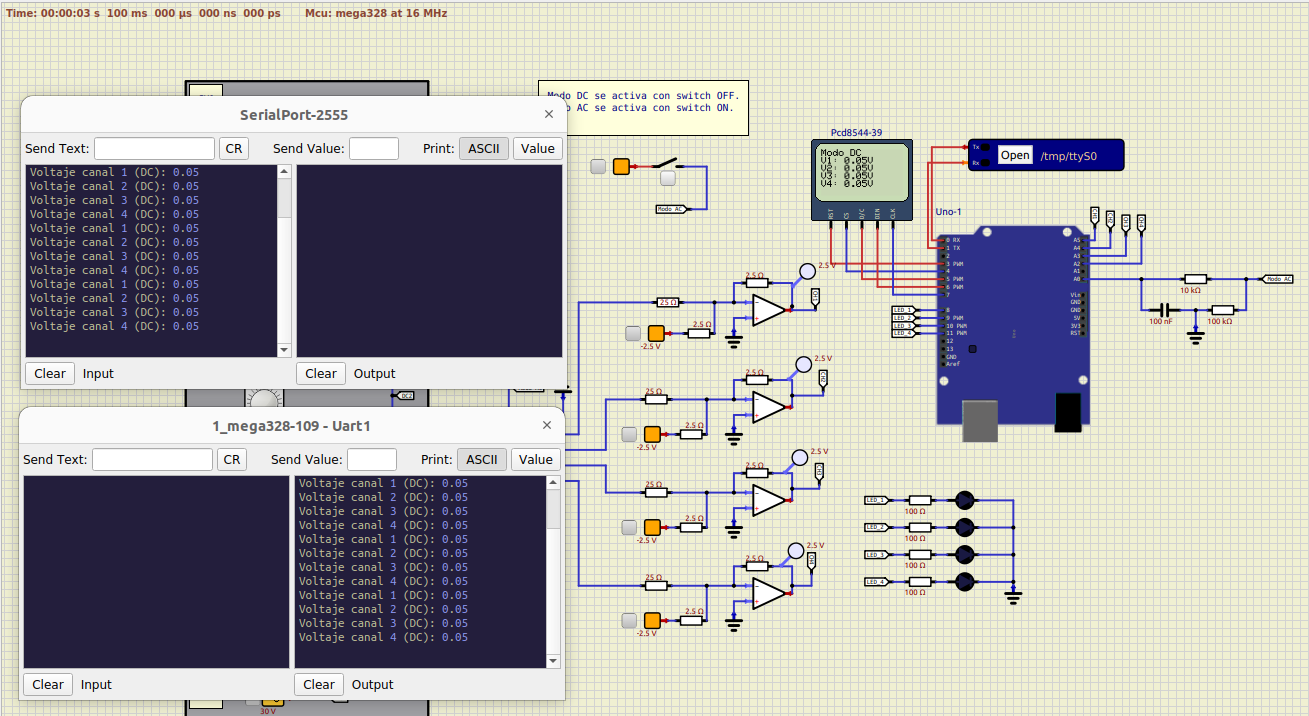
\includegraphics[width=.8\linewidth]{Imagenes/8a.png}
    \caption{Verificación de la comunicación entre el arduino y el puerto serial.}
    \label{figk2}
\end{figure}
Una vez comprobado el funcionamiento correcto de la comunicación anterior se procede a crear un puerto virtual para que pueda haber intercambio de información entre el puerto serial y el puerto serial virtual, S1, para ello se debe correr el bash script con el siguiente comando:\\
\textit{socat PTY,link=/tmp/ttyS0,raw,echo=0 PTY,link=/tmp/ttyS1,raw,echo}\\
Con este comando se crea el puerto virtual necesario, por lo que finalmente se procede a escribir un programa sencillo en python encargado de abrir un archivo csv y escribir en ello los datos correspondientes del puerto serial.\\
Los pasos para correr todo entonces es, primero correr el bash script, seguidamente abrir la comunicación en el simulador haciendo click en la opción de ''Open'', correr el script de python y finalmente correr la simulación, basado en este proceso se obtienen los siguientes resultados:
\begin{figure}[H]
    \centering
    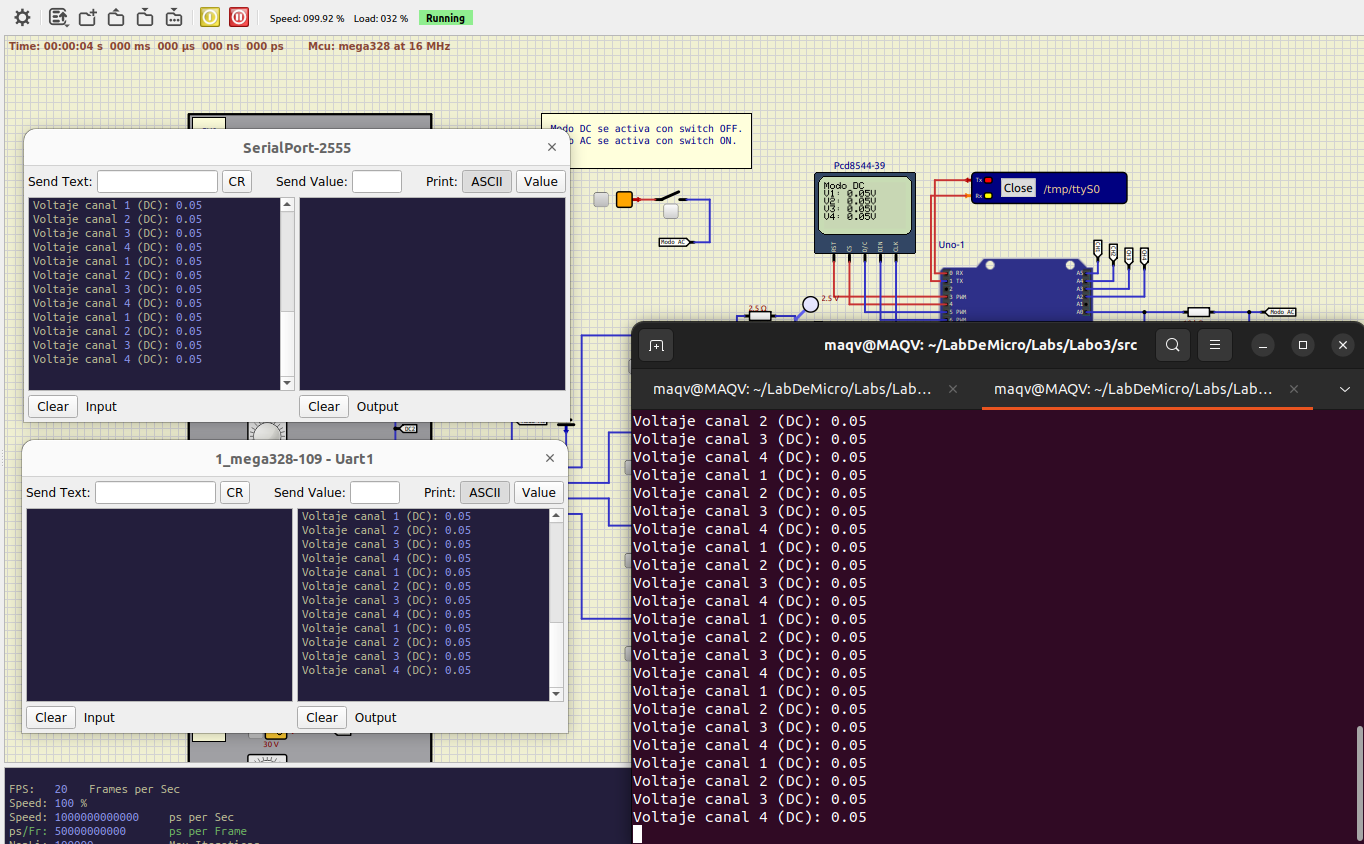
\includegraphics[width=.8\linewidth]{Imagenes/8b.png}
    \caption{Verificación de la comunicación entre el puerto serial y el puerto virtual.}
    \label{figk3}
\end{figure}
Ya se comprobó la generación correcta de los archivos csv, con sus respectivos valores, pero si se quisiera verificar se puede correr con el mismo con los archivos encontrados en el repositorio al igual el switch usado para la transmisión serial.\\
https://github.com/JosueC07183/Labo3.git

\newpage